\documentclass[11pt]{article}
\usepackage[a4paper,margin=2.2cm]{geometry}
\usepackage[utf8]{inputenc}
\usepackage[T1]{fontenc}
\usepackage[french]{babel}
\usepackage{graphicx}
\usepackage{booktabs}
\usepackage{longtable}
\usepackage{array}
\usepackage{xcolor}
\usepackage{hyperref}
\usepackage{fancyhdr}
\usepackage{titlesec}
\usepackage{amssymb}

\definecolor{accentcolor}{HTML}{0891B2}
\definecolor{emeraldcolor}{HTML}{10B981}
\hypersetup{colorlinks=true, linkcolor=accentcolor, urlcolor=accentcolor, citecolor=accentcolor}
\titleformat{\section}{\Large\bfseries\color{accentcolor}}{\thesection}{1em}{}
\titleformat{\subsection}{\large\bfseries}{\thesubsection}{1em}{}

\pagestyle{fancy}
\fancyhf{}
\fancyhead[L]{Jumeau Numérique CDU \& Vapocraqueur}
\fancyhead[R]{\thepage}
\renewcommand{\headrulewidth}{0.4pt}

% Chemin des images collectees dans ce meme dossier "images/"
\graphicspath{{images/}}

\newcommand{\okmark}{\textcolor{emeraldcolor}{\ding{51}}}
\usepackage{pifont}

\title{\textbf{Optimisation du Raffinage et de la Pétrochimie par Deep Learning}\\
\large Rapport de projet — Jumeau numérique CDU \& Vapocraqueur}
\author{}
\date{}

\begin{document}
\maketitle
\thispagestyle{fancy}

\section{Le problème}

Une raffinerie traitant \textbf{200 000 barils/jour} exploite une unité de distillation
atmosphérique (\textbf{CDU}) et un \textbf{vapocraqueur}, deux goulets d'étranglement du site.
L'objectif est de construire un système capable de :

\begin{enumerate}
  \item \textbf{Prédire les rendements des coupes} (naphta, kérosène, gazole, résidu)
  \item \textbf{Détecter les dérives opérationnelles et le fouling} (encrassement des échangeurs)
  \item \textbf{Optimiser les paramètres de distillation} (température du four, pression, reflux)
  \item \textbf{Réduire la consommation énergétique de 5-10 \%}
  \item \textbf{Prédire la qualité produit} et \textbf{alerter en temps réel}
\end{enumerate}

\begin{table}[h]
\centering
\begin{tabular}{clll}
\toprule
\# & Objectif & Critère de succès \\
\midrule
1 & Prédire les rendements & MAPE < 5 \% par coupe \\
2 & Détecter le fouling & Détection > 24 h avant nettoyage nécessaire \\
3 & Optimiser la température du four & Gain énergétique > 5 \% \\
4 & Prédire la qualité des produits & Corrélation > 0.9 avec le labo \\
5 & Déployer un système d'alerte & Temps réel (< 1 min) \\
\bottomrule
\end{tabular}
\caption{Objectifs et critères de succès}
\end{table}

Toutes les données sont \textbf{100 \% synthétiques}, générées à partir de bilans matière et
énergétiques d'une CDU et d'un vapocraqueur (\texttt{src/data\_generator.py}) — 2 ans de données
horaires ($\approx$17 500 points), plus un échantillonnage labo toutes les 8 h avec 4 h de délai.

\textbf{Contrainte de méthode : Deep Learning uniquement.} Aucun algorithme de ML classique
(XGBoost, Random Forest, régression linéaire/logistique, SVM, k-means...) — uniquement des
réseaux de neurones PyTorch. scikit-learn n'est utilisé que pour \texttt{StandardScaler}, les
métriques et le split train/val/test.

\section{Techniques de Deep Learning utilisées — étude comparative}

\begin{table}[h]
\centering
\begin{tabular}{p{3cm}p{6cm}p{5cm}}
\toprule
Famille & Modèles & Utilisés pour \\
\midrule
Dense & MLP & Baseline rendements, surrogate énergétique \\
Récurrent & RNN simple, LSTM, GRU, LSTM bidirectionnel & Rendements, soft sensor qualité, résidu de fouling \\
Convolutionnel & CNN 1D, TCN (dilaté causal) & Rendements \\
Hybride & CNN-LSTM & Disponible (\texttt{src/models/cnn.py}) \\
Attention & Transformer encoder & Rendements \\
Non supervisé & Autoencodeur dense, conv1D, LSTM seq2seq, VAE & Détection de fouling \\
Optimisation & Surrogate MLP + gradient sur les entrées & Optimisation énergétique \\
\bottomrule
\end{tabular}
\caption{Familles de réseaux de neurones utilisées}
\end{table}

\begin{table}[h]
\centering
\begin{tabular}{p{3cm}p{5.5cm}p{5.5cm}}
\toprule
Architecture & Avantage principal & Limite observée \\
\midrule
\textbf{RNN simple} & Meilleur compromis biais/variance ici ; peu de paramètres & Mémoire courte \\
LSTM / GRU / BiLSTM & Mémoire longue via portes & Sur-paramétrés ici (peu de gain) \\
TCN & Champ réceptif large, parallélisable & Sensible au nombre de blocs \\
Transformer & Dépendances globales via attention & Plus lent, besoin de plus de données \\
CNN 1D & Rapide, motifs locaux & Moins adapté aux dépendances longues \\
MLP (baseline) & Simple, rapide & Ignore l'historique temporel \\
\bottomrule
\end{tabular}
\caption{Comparatif qualitatif (notebook 03, tâche rendements)}
\end{table}

Sur ce jeu de données (fenêtres de 24 h), les architectures \textbf{plus simples} (RNN, TCN,
MLP) égalent voire dépassent les architectures plus complexes — signe que la tâche ne
nécessite pas une mémoire très longue. Pour le fouling, les \textbf{autoencodeurs} (entraînés
sur périodes propres) détectent une dérive via l'erreur de reconstruction ; l'approche par
\textbf{résidu GRU} surveille l'écart mesuré/prédit d'un capteur clé. Pour l'énergie, un
\textbf{réseau surrogate} différentiable permet une \textbf{descente de gradient sur les
entrées} (COT, reflux).

\section{Résultats détaillés par notebook}

\subsection{Notebooks 01-02 — Exploration et préprocessing}

Statistiques descriptives, valeurs manquantes/outliers injectés, cycle de fouling (4
nettoyages/2 ans), STL, ACF/PACF. Préprocessing : imputation temporelle, correction de dérive
capteur, jointure asof labo (délai 4h, zéro fuite), split temporel strict 70/15/15.

\begin{figure}[h]
\centering
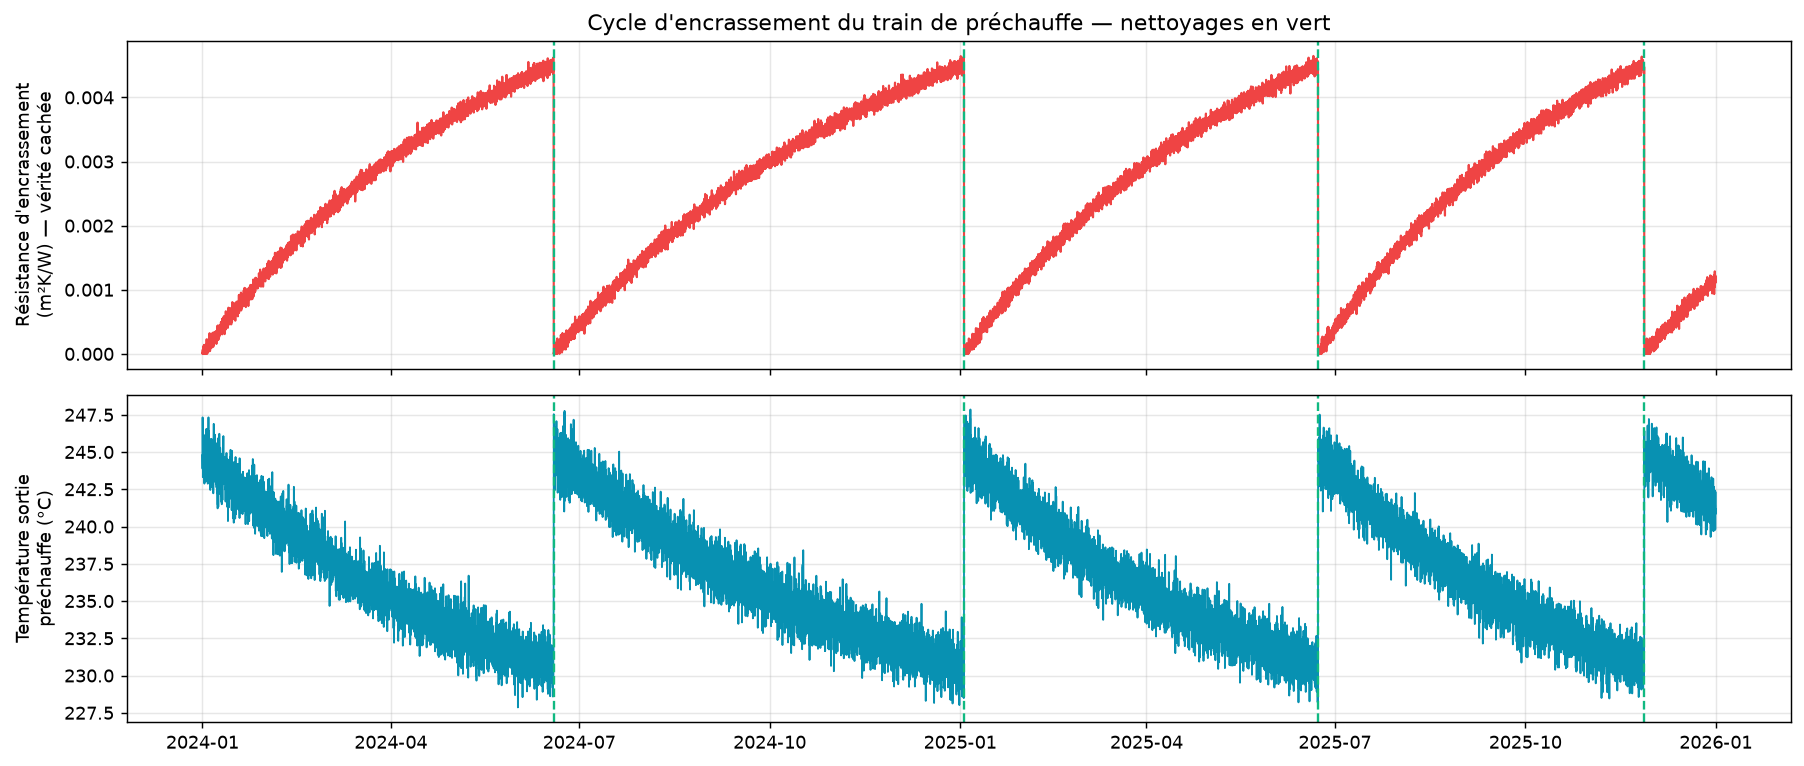
\includegraphics[width=0.85\textwidth]{01_cycle_fouling.png}
\caption{Cycle de fouling — résistance cachée et nettoyages}
\end{figure}

\subsection{Notebook 03 — Prédiction des rendements (8 architectures)}

\begin{table}[h]
\centering
\small
\begin{tabular}{lrrrrrrr}
\toprule
Architecture & Naphta & Kéro. & Gazole & Résidu & \textbf{Global} & Params & Temps (s) \\
\midrule
\textbf{RNN simple} & 4.95\% & 1.82\% & 1.12\% & 4.06\% & \textbf{2.99\%} & 13 956 & 52.9 \\
TCN & 5.30\% & 2.16\% & 1.24\% & 4.32\% & 3.26\% & 42 884 & 103.1 \\
MLP (baseline) & 5.37\% & 2.24\% & 1.22\% & 4.20\% & 3.26\% & 19 652 & 24.1 \\
LSTM & 5.37\% & 2.23\% & 1.25\% & 4.31\% & 3.29\% & 75 844 & 114.4 \\
LSTM bidirectionnel & 5.52\% & 2.12\% & 1.28\% & 4.43\% & 3.34\% & 184 132 & 185.8 \\
GRU & 5.76\% & 2.29\% & 1.25\% & 4.28\% & 3.40\% & 57 988 & 161.5 \\
Transformer & 6.06\% & 2.38\% & 1.42\% & 4.41\% & 3.57\% & 74 660 & 314.7 \\
CNN 1D & 6.85\% & 2.67\% & 1.74\% & 5.49\% & 4.19\% & 29 092 & 79.4 \\
\bottomrule
\end{tabular}
\caption{MAPE par coupe et global — 8 architectures (notebook 03)}
\end{table}

\textbf{Résultat : objectif MAPE < 5\% atteint (RNN simple, 2.99\% global). \checkmark}

\begin{figure}[h]
\centering
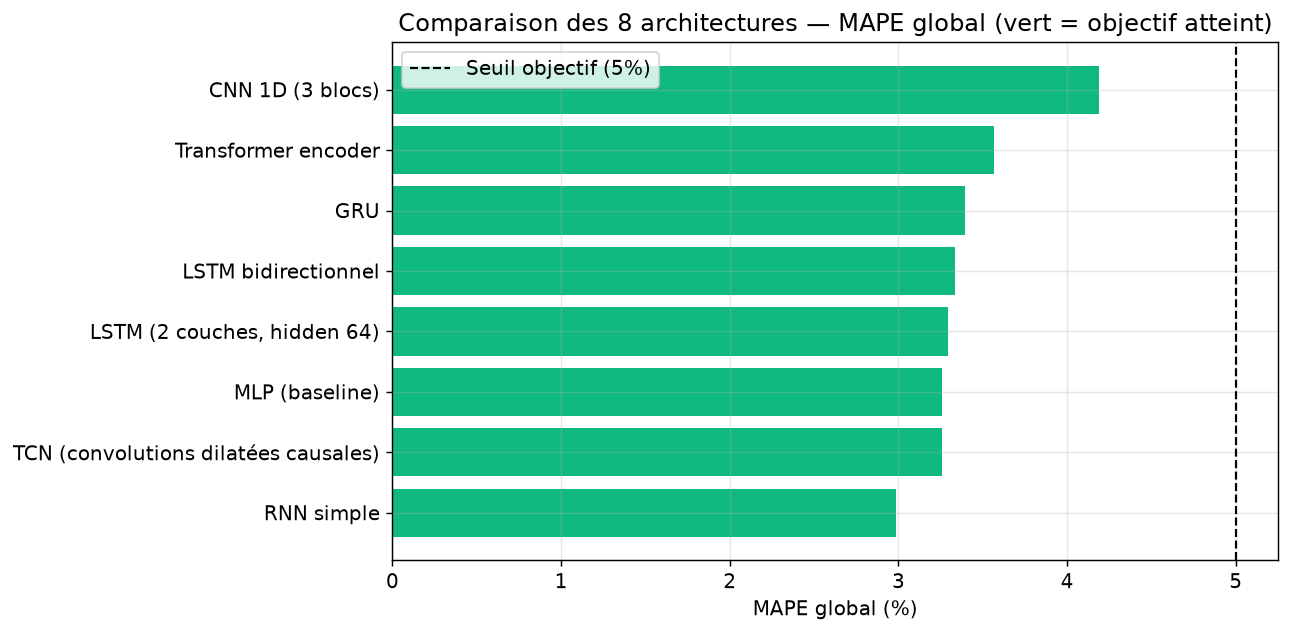
\includegraphics[width=0.85\textwidth]{03_comparaison_architectures.png}
\caption{Comparatif des 8 architectures — MAPE global}
\end{figure}

\begin{figure}[h]
\centering
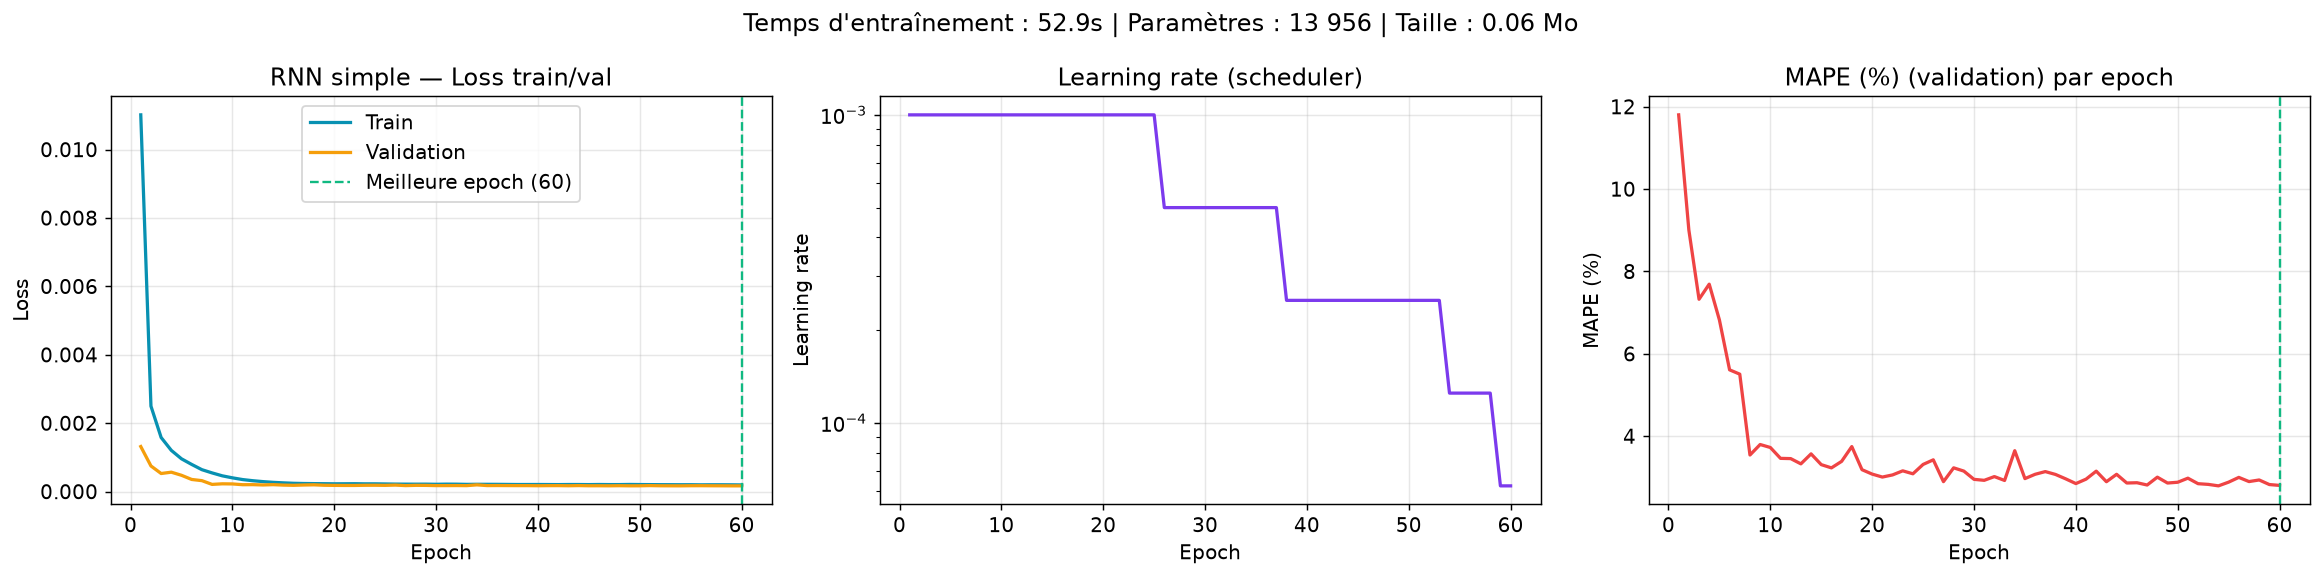
\includegraphics[width=0.85\textwidth]{03_learning_curve_rnn.png}
\caption{Courbe d'apprentissage — RNN simple (architecture retenue)}
\end{figure}

\begin{figure}[h]
\centering
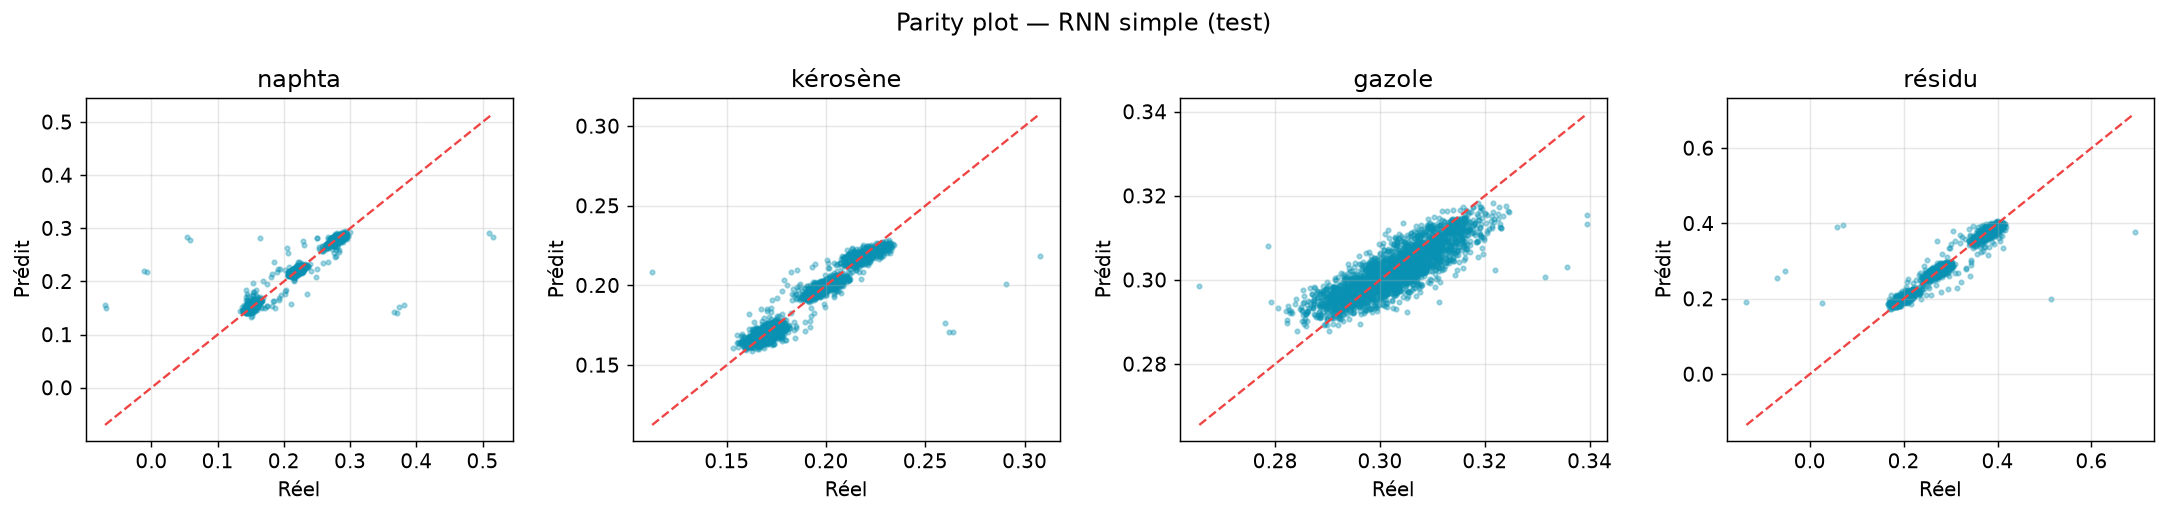
\includegraphics[width=0.85\textwidth]{03_parity_plot.png}
\caption{Parity plot — meilleur modèle}
\end{figure}

\begin{figure}[h]
\centering
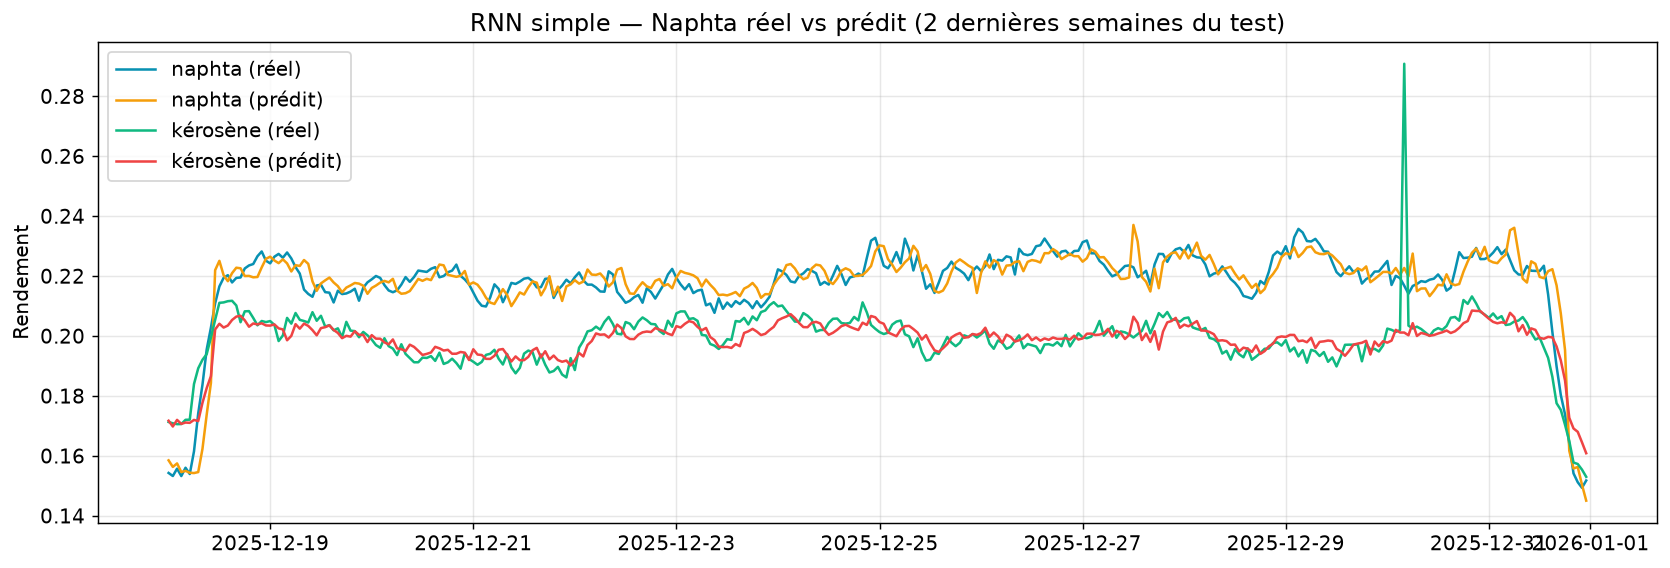
\includegraphics[width=0.85\textwidth]{03_pred_vs_reel_2semaines.png}
\caption{Prédit vs réel sur 2 semaines de test}
\end{figure}

\begin{figure}[h]
\centering
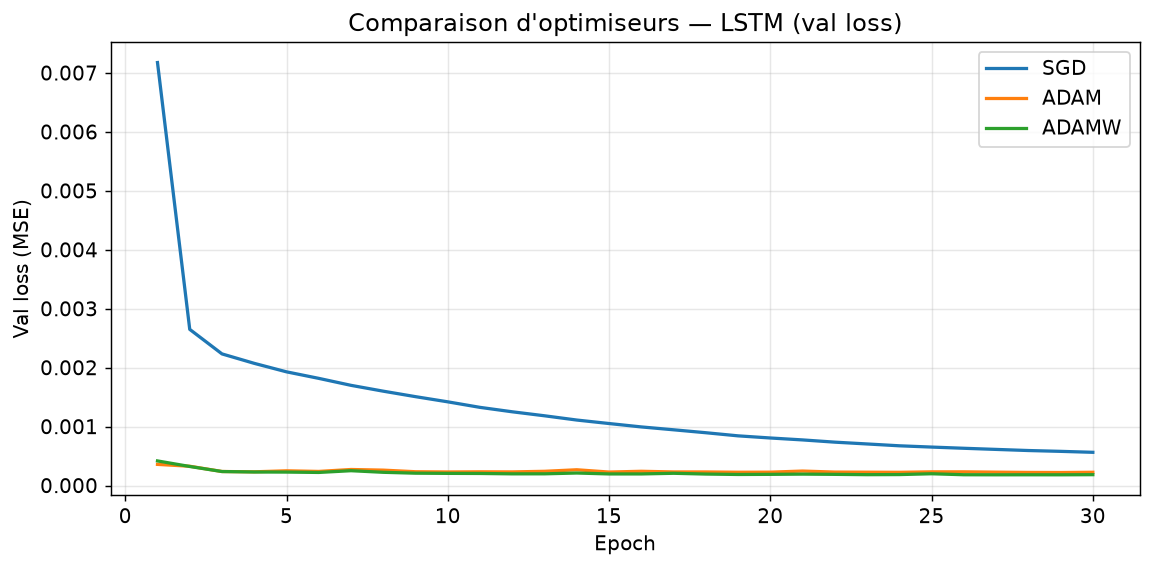
\includegraphics[width=0.7\textwidth]{03_optimizer_comparison.png}
\caption{Comparaison d'optimiseurs (SGD / Adam / AdamW)}
\end{figure}

\begin{figure}[h]
\centering
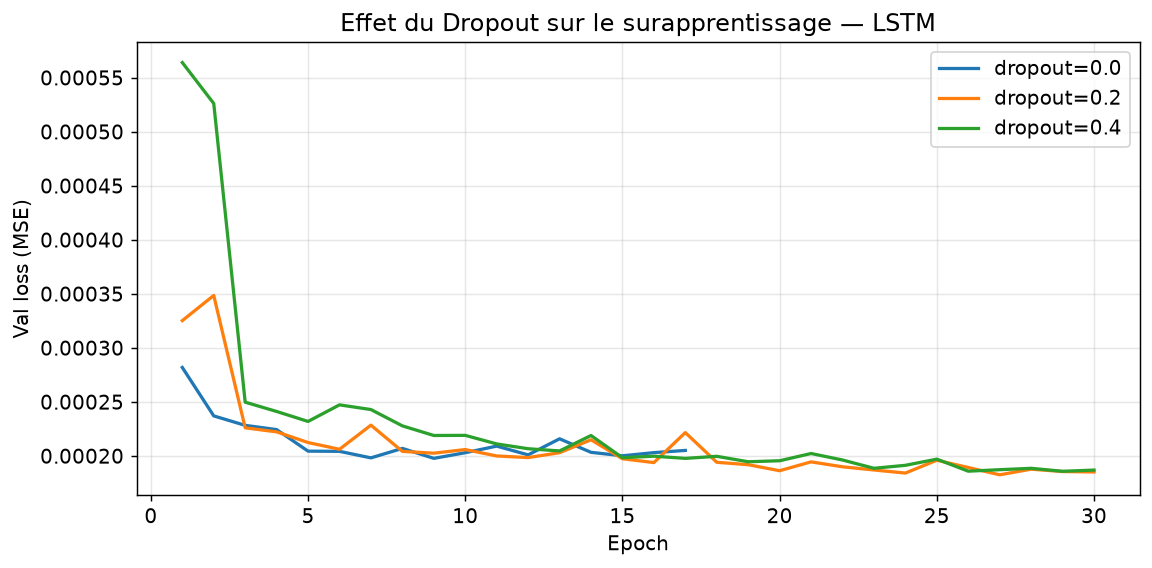
\includegraphics[width=0.7\textwidth]{03_dropout_comparison.png}
\caption{Effet du dropout (0.0 / 0.2 / 0.4) sur le sur-apprentissage}
\end{figure}

\subsection{Notebook 04 — Détection du fouling (5 approches)}

\begin{table}[h]
\centering
\small
\begin{tabular}{lrrrrrr}
\toprule
Méthode & Precision & Recall & F1 & AUC & \textbf{Avance (h)} & Params \\
\midrule
Autoencodeur dense & 0.032 & 0.542 & 0.060 & 0.765 & \textbf{3764} & 516 128 \\
Autoencodeur LSTM & 0.012 & 0.583 & 0.024 & 0.633 & 4129 & 26 163 \\
VAE & 0.012 & 0.219 & 0.024 & 0.712 & 3414 & 259 808 \\
Autoencodeur conv1D & 0.011 & 0.615 & 0.022 & 0.624 & 3851 & 19 331 \\
Résidu GRU & 0.009 & 0.323 & 0.018 & 0.676 & 2972 & 57 793 \\
\bottomrule
\end{tabular}
\caption{Comparatif des 5 approches de détection de fouling (notebook 04)}
\end{table}

\textbf{Résultat : les 5 méthodes dépassent l'objectif de 24h. \checkmark} Précision faible
pour toutes (fort déséquilibre de classes, $\sim$0.9\% d'heures positives) mais rappel et AUC
démontrent un pouvoir de détection réel. \textbf{Production : autoencodeur dense.}

\begin{figure}[h]
\centering
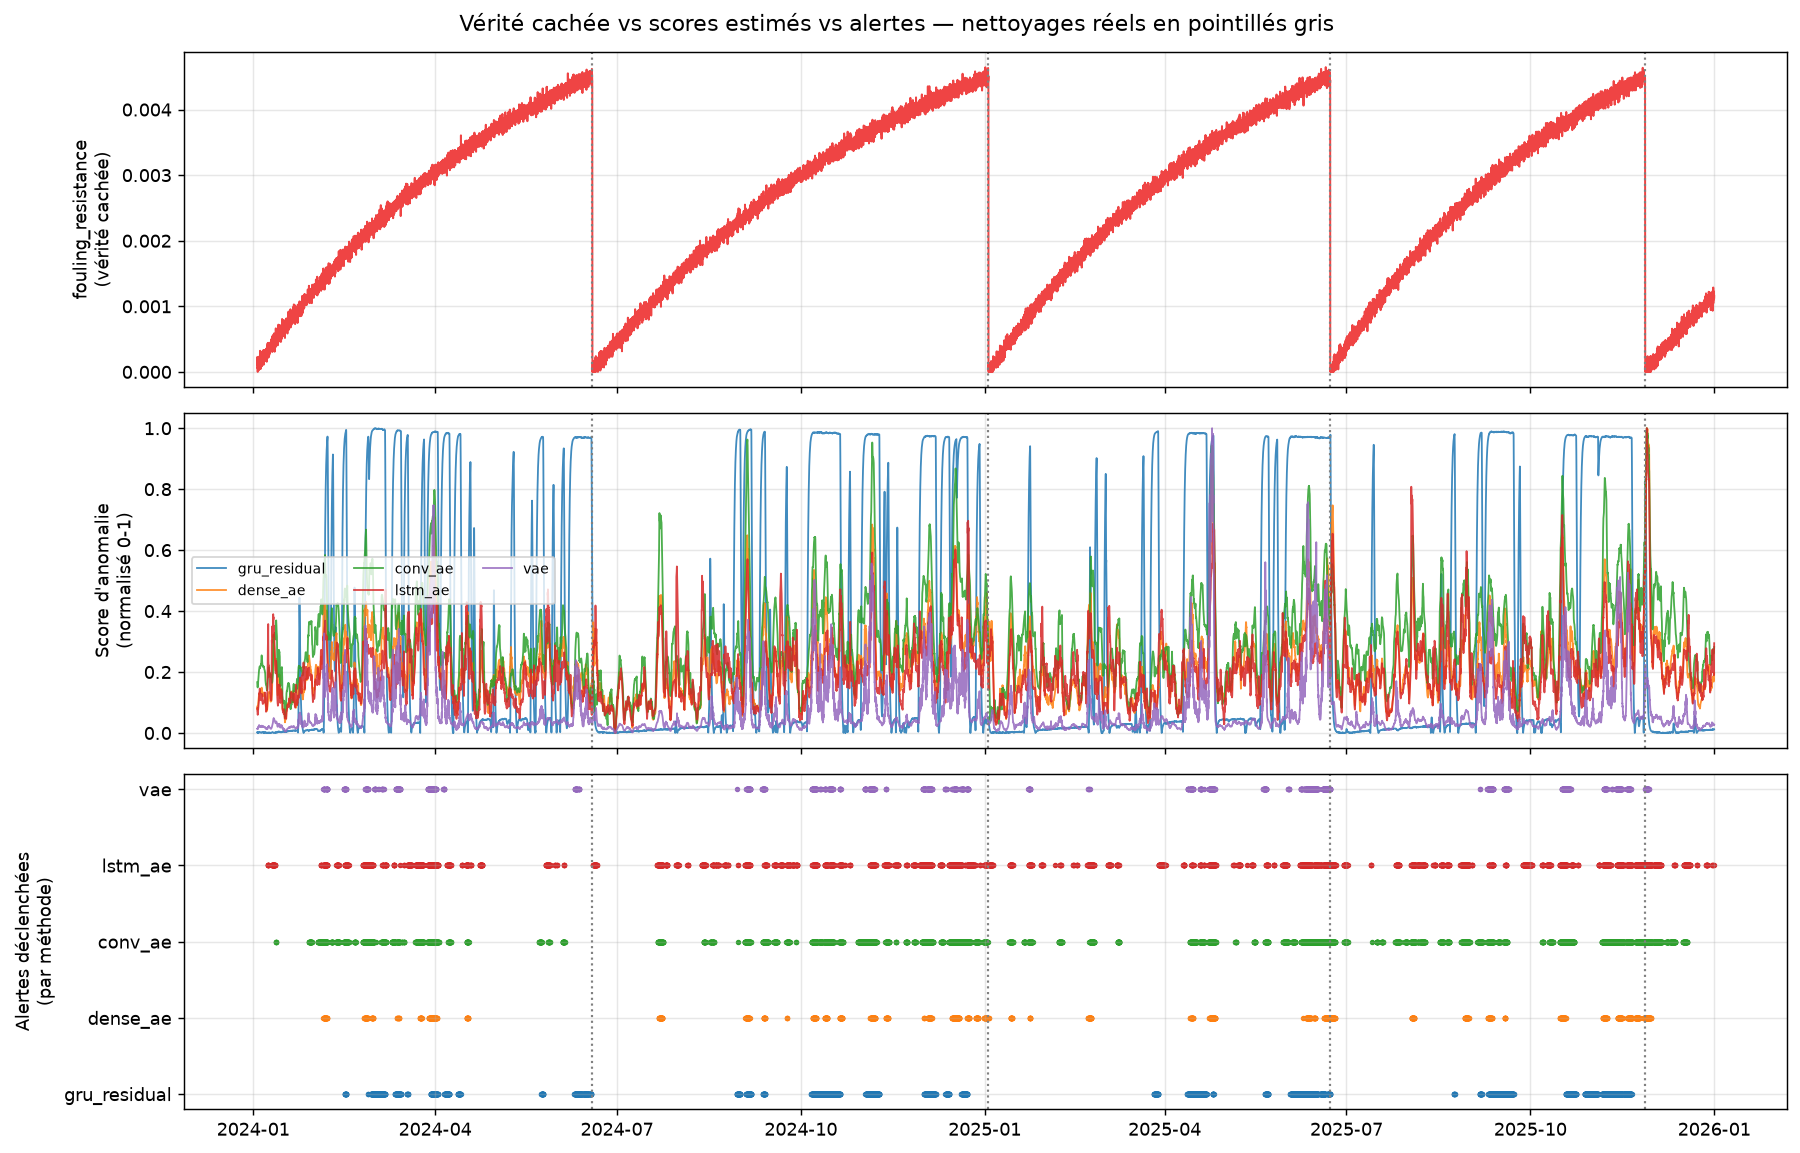
\includegraphics[width=0.85\textwidth]{04_timeline_verite_vs_detections.png}
\caption{Timeline : vérité cachée vs indices estimés vs alertes}
\end{figure}

\begin{figure}[h]
\centering
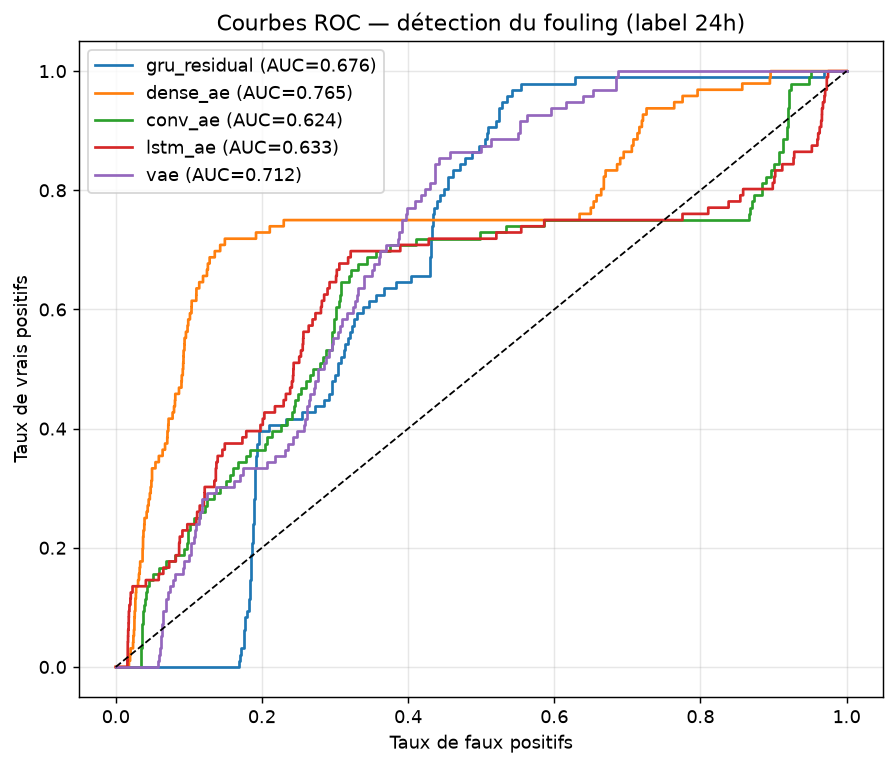
\includegraphics[width=0.7\textwidth]{04_roc_curves.png}
\caption{Courbes ROC des 5 méthodes}
\end{figure}

\begin{figure}[h]
\centering
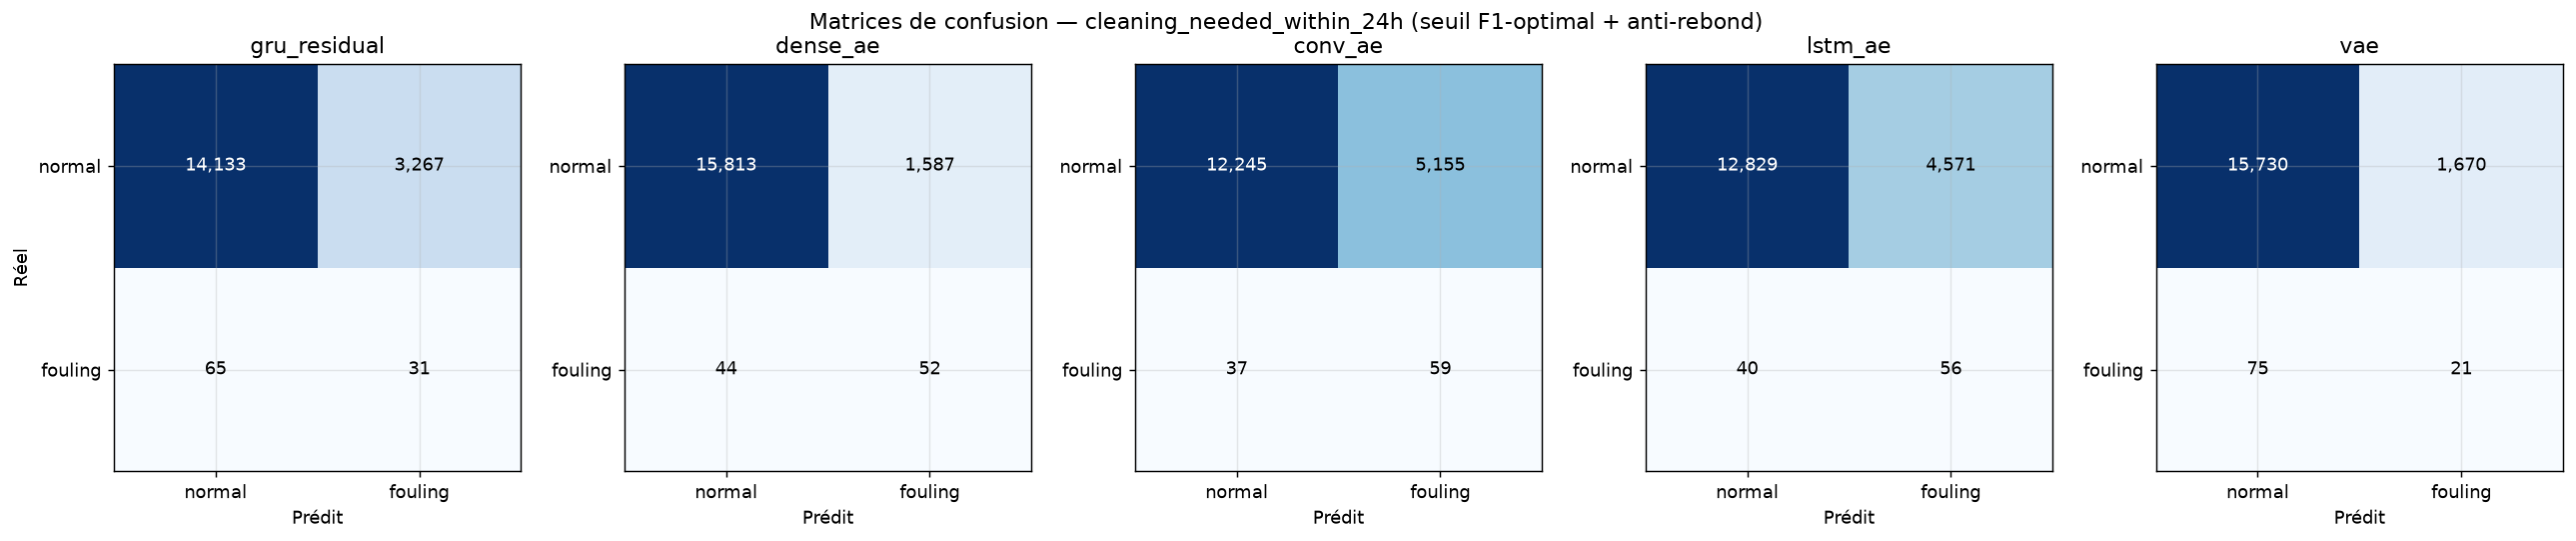
\includegraphics[width=\textwidth]{04_confusion_matrices.png}
\caption{Matrices de confusion (label cleaning\_needed\_within\_24h)}
\end{figure}

\begin{figure}[h]
\centering
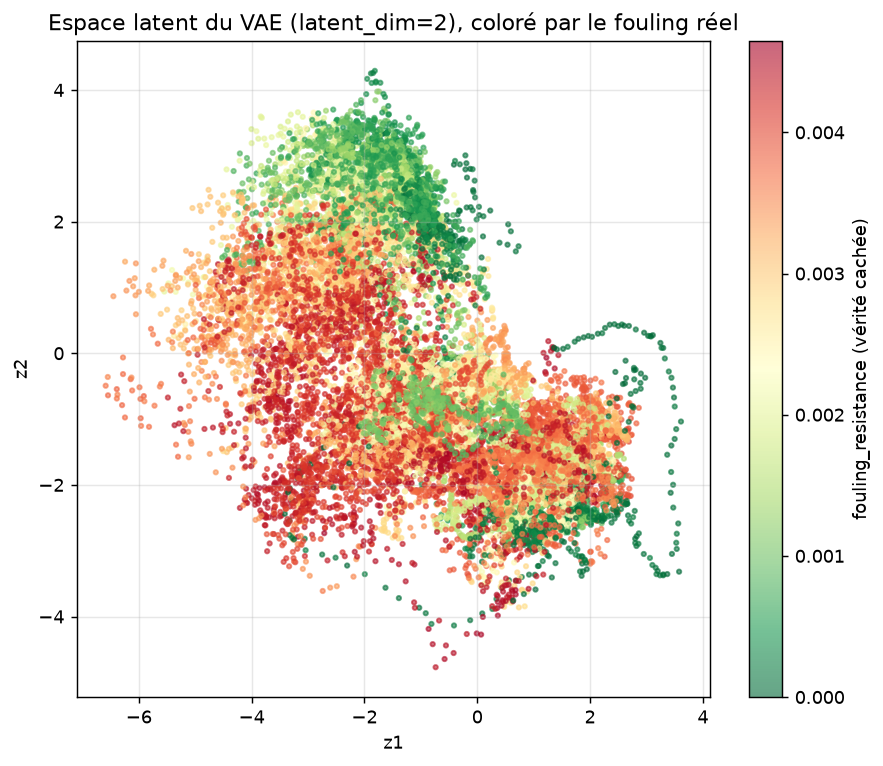
\includegraphics[width=0.7\textwidth]{04_vae_latent_space.png}
\caption{Espace latent du VAE (projection 2D)}
\end{figure}

\subsection{Notebook 05 — Optimisation énergétique}

Surrogate MLP (128-128-64) prédisant (4 rendements + énergie spécifique). Optimisation par
descente de gradient sur COT/reflux, poids gelés, sous contrainte de préservation des rendements.

\begin{table}[h]
\centering
\begin{tabular}{lr}
\toprule
Métrique & Valeur \\
\midrule
Gain énergétique (gradient) & \textbf{5.53 \%} \checkmark (objectif > 5\%) \\
Comparaison random search & 7.68 \% (sans garantie des contraintes) \\
Respect de la contrainte de rendement & 96.3 \% des échantillons \\
Économies & $\approx$ 774 \$/jour, 4.13 tCO$_2$/jour évitées \\
\bottomrule
\end{tabular}
\caption{Résultats de l'optimisation énergétique (notebook 05)}
\end{table}

\begin{figure}[h]
\centering

\includegraphics[width=0.7\textwidth]{05_learning_curve_surrogate.png}
\caption{Courbe d'apprentissage du surrogate}
\end{figure}

\begin{figure}[h]
\centering
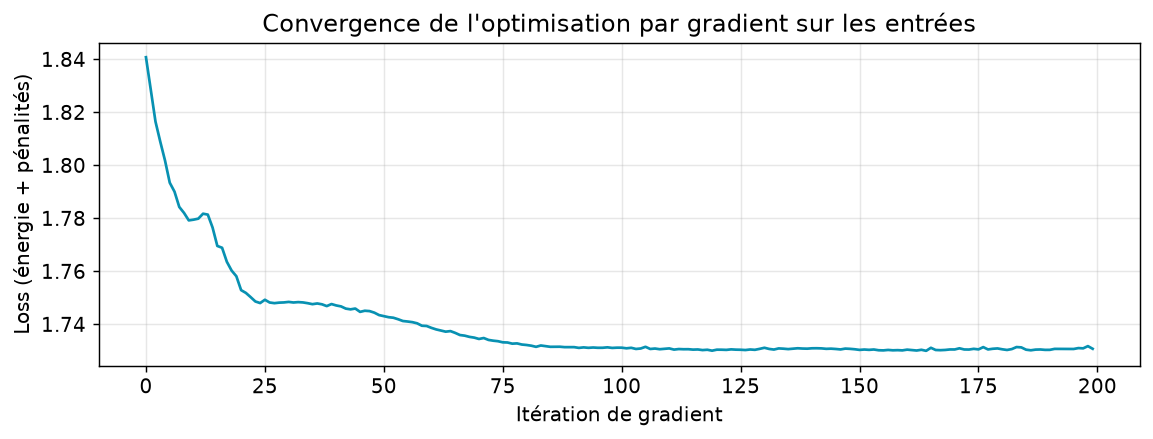
\includegraphics[width=0.7\textwidth]{05_convergence_gradient.png}
\caption{Convergence de l'optimisation par gradient}
\end{figure}

\begin{figure}[h]
\centering
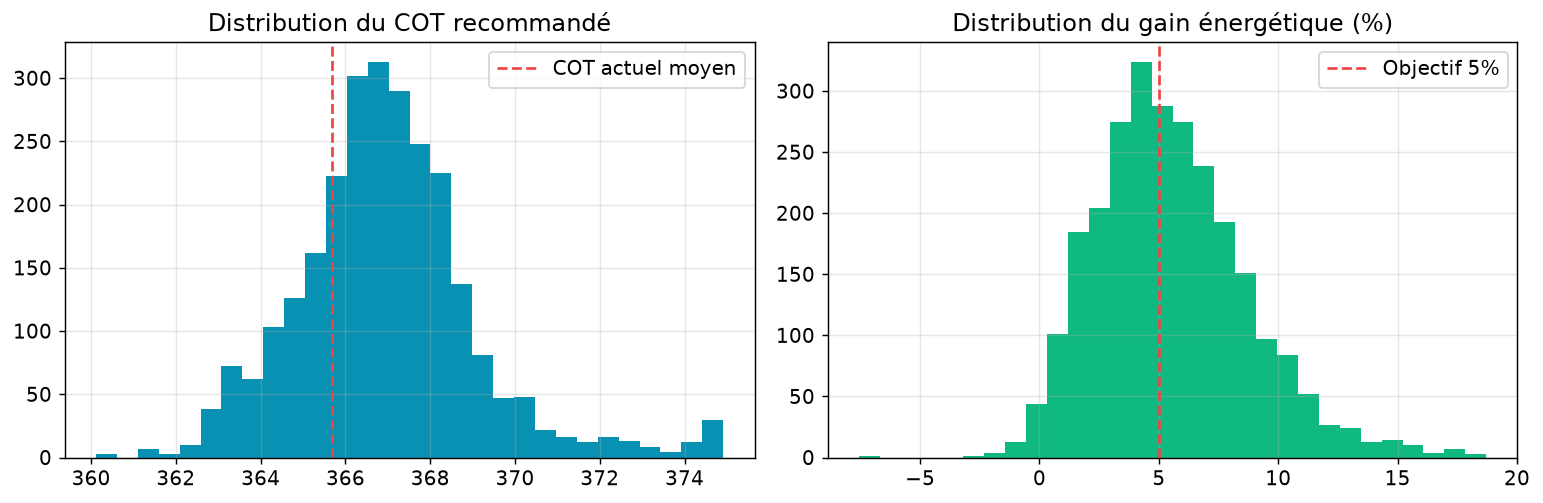
\includegraphics[width=0.85\textwidth]{05_optimisation_resultats.png}
\caption{Distribution des recommandations COT et des gains}
\end{figure}

\subsection{Notebook 06 — Soft sensor qualité + pipeline temps réel}

GRU multi-sorties (5 cibles qualité labo), cibles standardisées séparément.

\begin{table}[h]
\centering
\begin{tabular}{lr}
\toprule
Cible qualité & Corrélation (test) \\
\midrule
Point final naphta & 0.966 \\
Point éclair kérosène & 0.965 \\
Indice de cétane gazole & 0.972 \\
Viscosité résidu & 0.967 \\
Teneur en soufre & 0.985 \\
\textbf{Moyenne} & \textbf{0.971} \checkmark (objectif > 0.9) \\
\bottomrule
\end{tabular}
\caption{Corrélations du soft sensor qualité (notebook 06)}
\end{table}

Pipeline temps réel : rejeu heure par heure (2633 h), 3 réseaux en inférence continue + moteur
d'alertes anti-rebond. \textbf{Latence moyenne mesurée : $\sim$55 ms} (objectif < 1 min). 116
alertes générées lors du backtest.

\begin{figure}[h]
\centering

\includegraphics[width=0.7\textwidth]{06_learning_curve_quality.png}
\caption{Courbe d'apprentissage — soft sensor qualité}
\end{figure}

\begin{figure}[h]
\centering
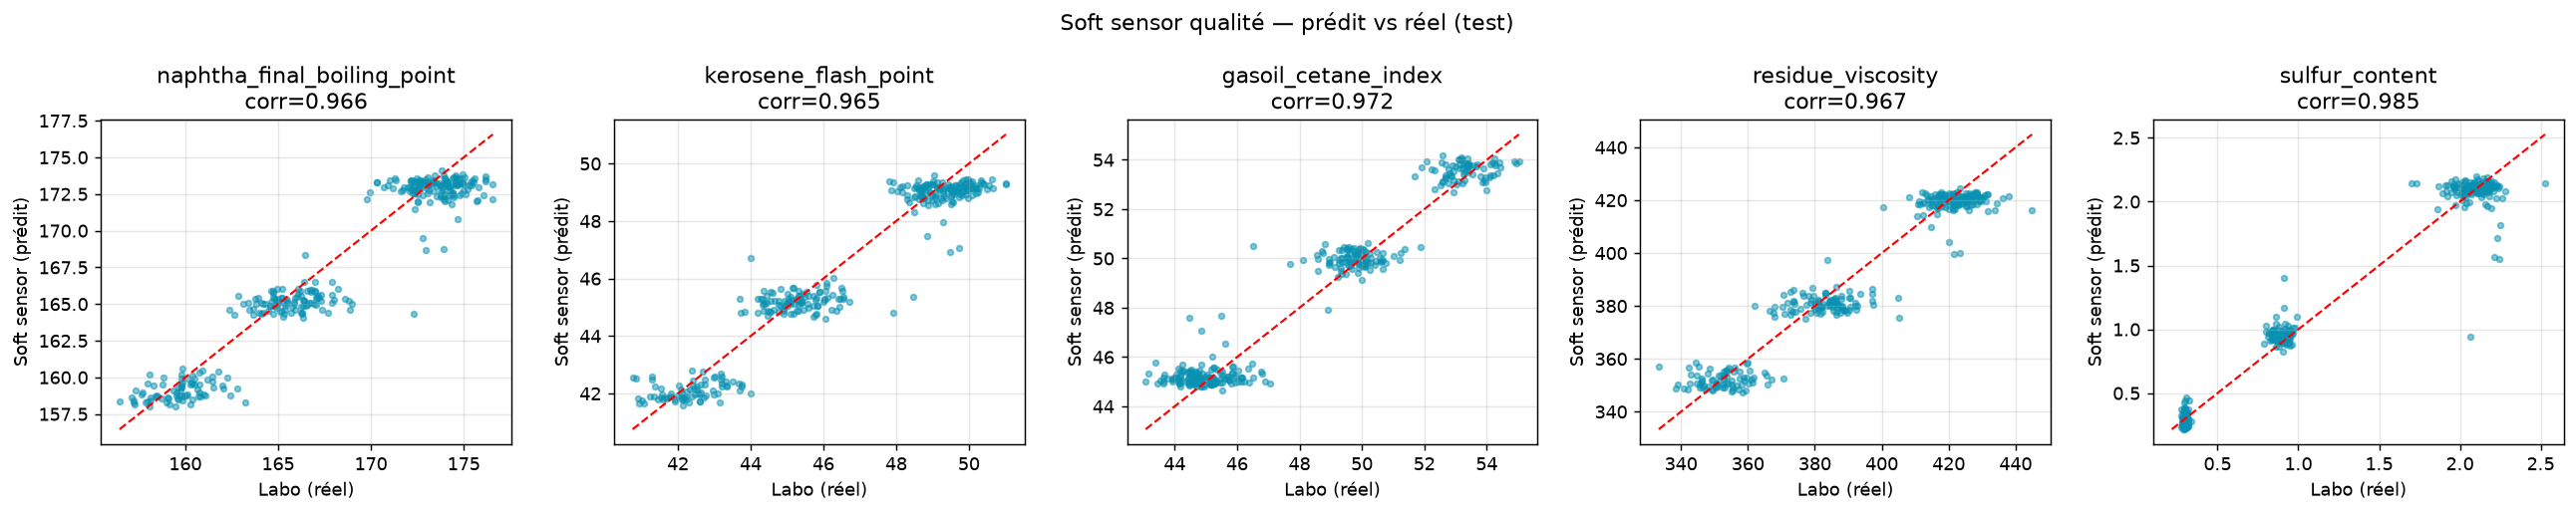
\includegraphics[width=0.85\textwidth]{06_quality_parity.png}
\caption{Prédit vs réel — soft sensor qualité (5 cibles)}
\end{figure}

\begin{figure}[h]
\centering

\includegraphics[width=0.85\textwidth]{06_latence_et_alertes.png}
\caption{Latence par tick et alertes générées}
\end{figure}

\subsection{Synthèse finale}

\begin{table}[h]
\centering
\begin{tabular}{clll}
\toprule
\# & Objectif & Résultat & Statut \\
\midrule
1 & Rendements (MAPE < 5\%) & 2.99\% (RNN simple) & \checkmark \\
2 & Fouling (> 24h) & 3764h (autoencodeur dense) & \checkmark \\
3 & Énergie (gain > 5\%) & 5.53\% (774\$/j, 4.13 tCO$_2$/j) & \checkmark \\
4 & Qualité (corr > 0.9) & 0.971 & \checkmark \\
5 & Alertes temps réel (< 1 min) & $\sim$55 ms (max 226 ms) & \checkmark \\
\bottomrule
\end{tabular}
\caption{5/5 objectifs atteints — rapport généré automatiquement (\texttt{model\_report.md})}
\end{table}

\section{Le dashboard — jumeau numérique}

\subsection{Ce qu'il fait}

Le dashboard consomme le backend FastAPI (\texttt{/api/*} + WebSocket \texttt{/ws/realtime}) qui
rejoue en continu le jeu de test (1h de données simulées par tick de 2s) à travers les 4
modèles de production (rendements, fouling, qualité, surrogate énergie), génère des alertes, et
diffuse un état complet (\texttt{TwinState}) à tous les clients connectés.

\begin{table}[h]
\centering
\begin{tabular}{p{3.5cm}p{11cm}}
\toprule
Page & Rôle \\
\midrule
Vue d'ensemble (\texttt{/}) & KPI temps réel, aire empilée des rendements (48h), flux d'alertes, compteurs de gains \\
Jumeau numérique (\texttt{/jumeau}) & Synoptique interactif (React Flow) : Brut $\to$ Dessaleur $\to$ Préchauffe $\to$ Four $\to$ Colonne $\to$ Vapocraqueur, capteurs live, santé des équipements \\
Rendements (\texttt{/rendements}) & Courbes prédit/réel, jauges MAPE, simulateur what-if \\
Encrassement (\texttt{/encrassement}) & Indice de fouling, délai avant nettoyage, timeline 2 ans \\
Énergie (\texttt{/energie}) & Comparaison énergie réelle vs optimisée, optimisation à la demande \\
Alertes (\texttt{/alertes}) & Journal filtrable des alertes \\
Documentation (\texttt{/documentation}) & Récapitulatif objectifs et architectures \\
\bottomrule
\end{tabular}
\caption{Pages du dashboard et leur rôle}
\end{table}

\subsection{Aperçu visuel}

\begin{figure}[h]
\centering
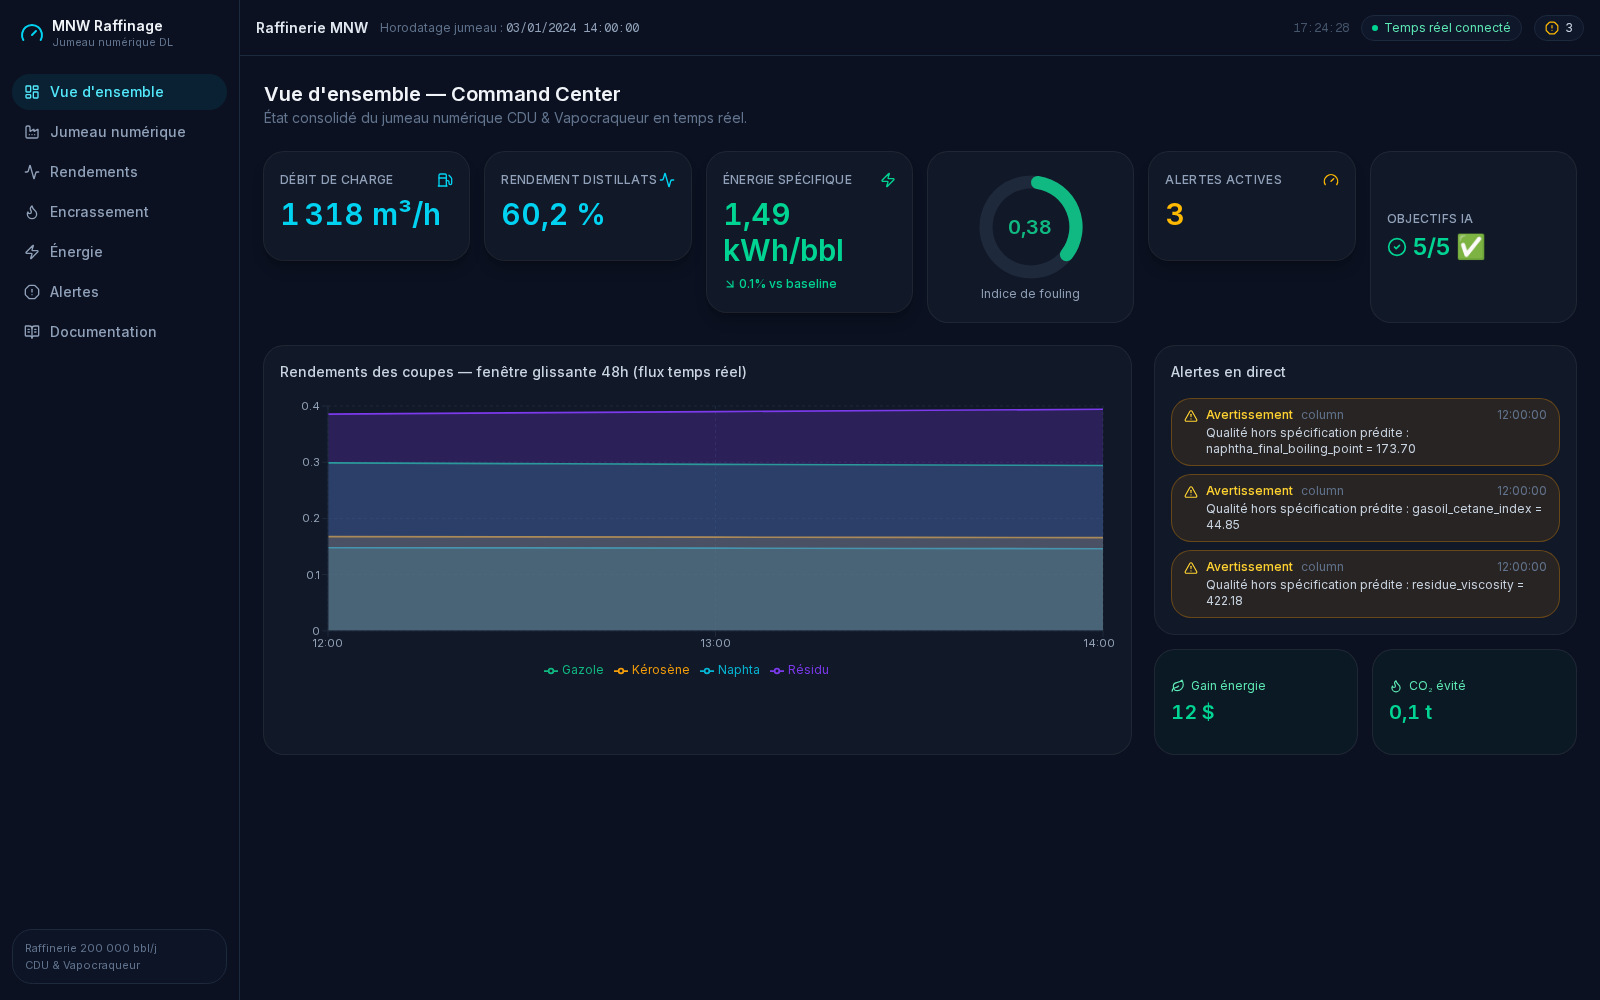
\includegraphics[width=0.85\textwidth]{dashboard_home.png}
\caption{Vue d'ensemble (Command Center)}
\end{figure}

\begin{figure}[h]
\centering
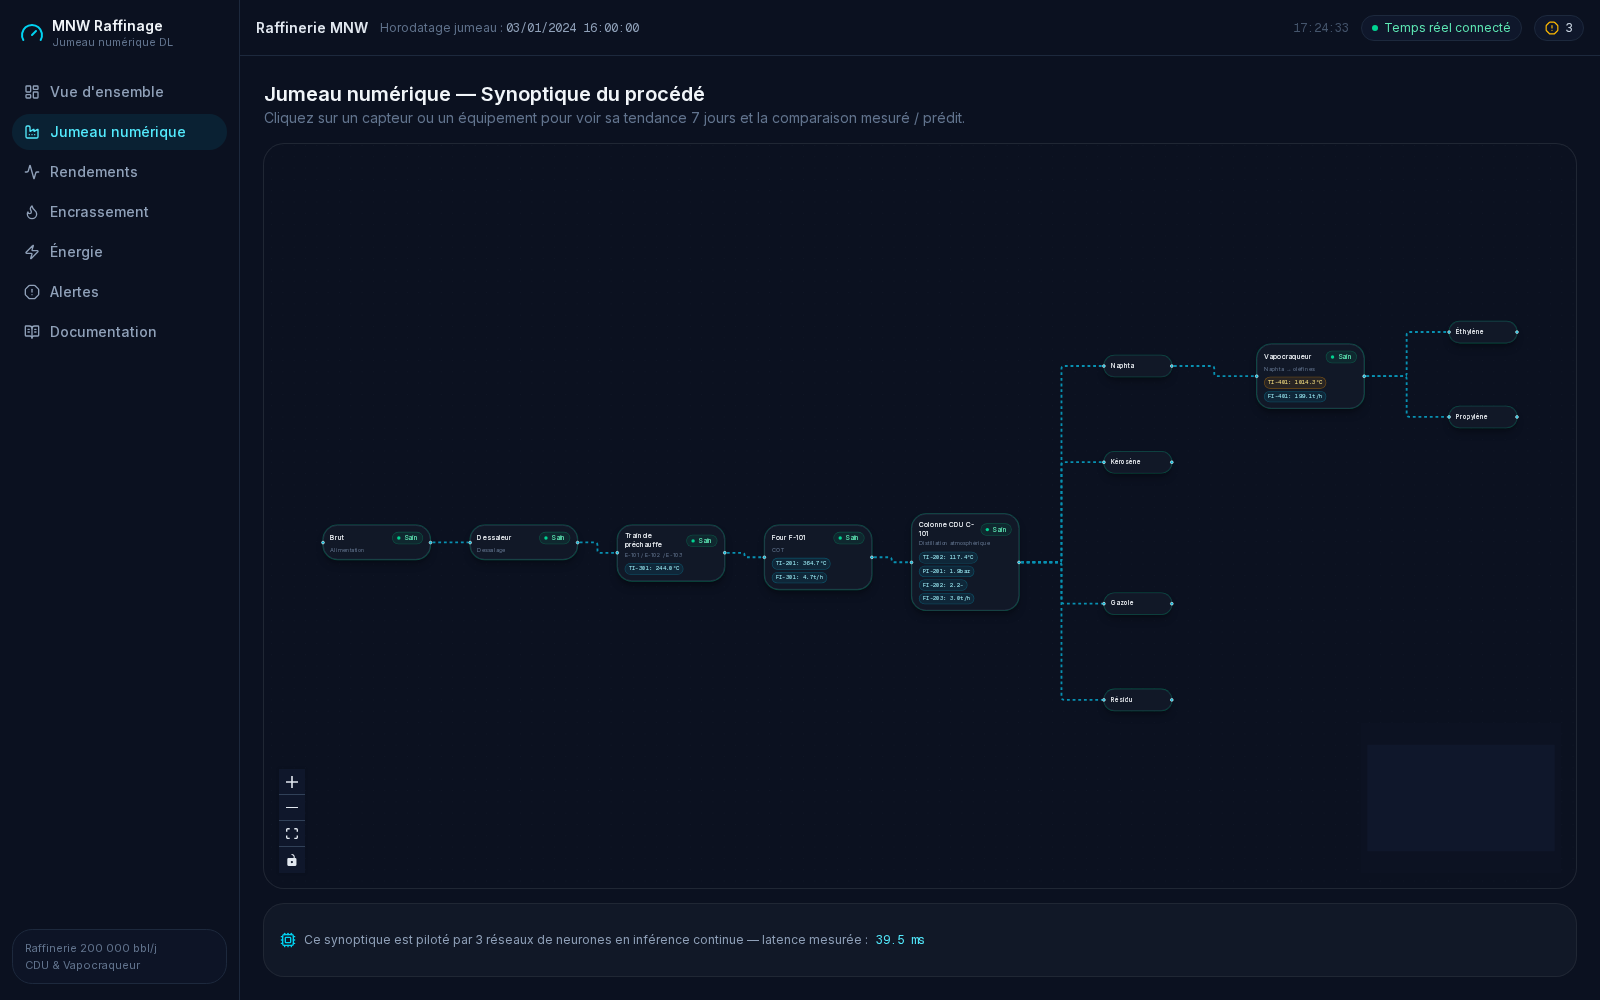
\includegraphics[width=0.85\textwidth]{dashboard_jumeau.png}
\caption{Synoptique du jumeau numérique}
\end{figure}

\begin{figure}[h]
\centering
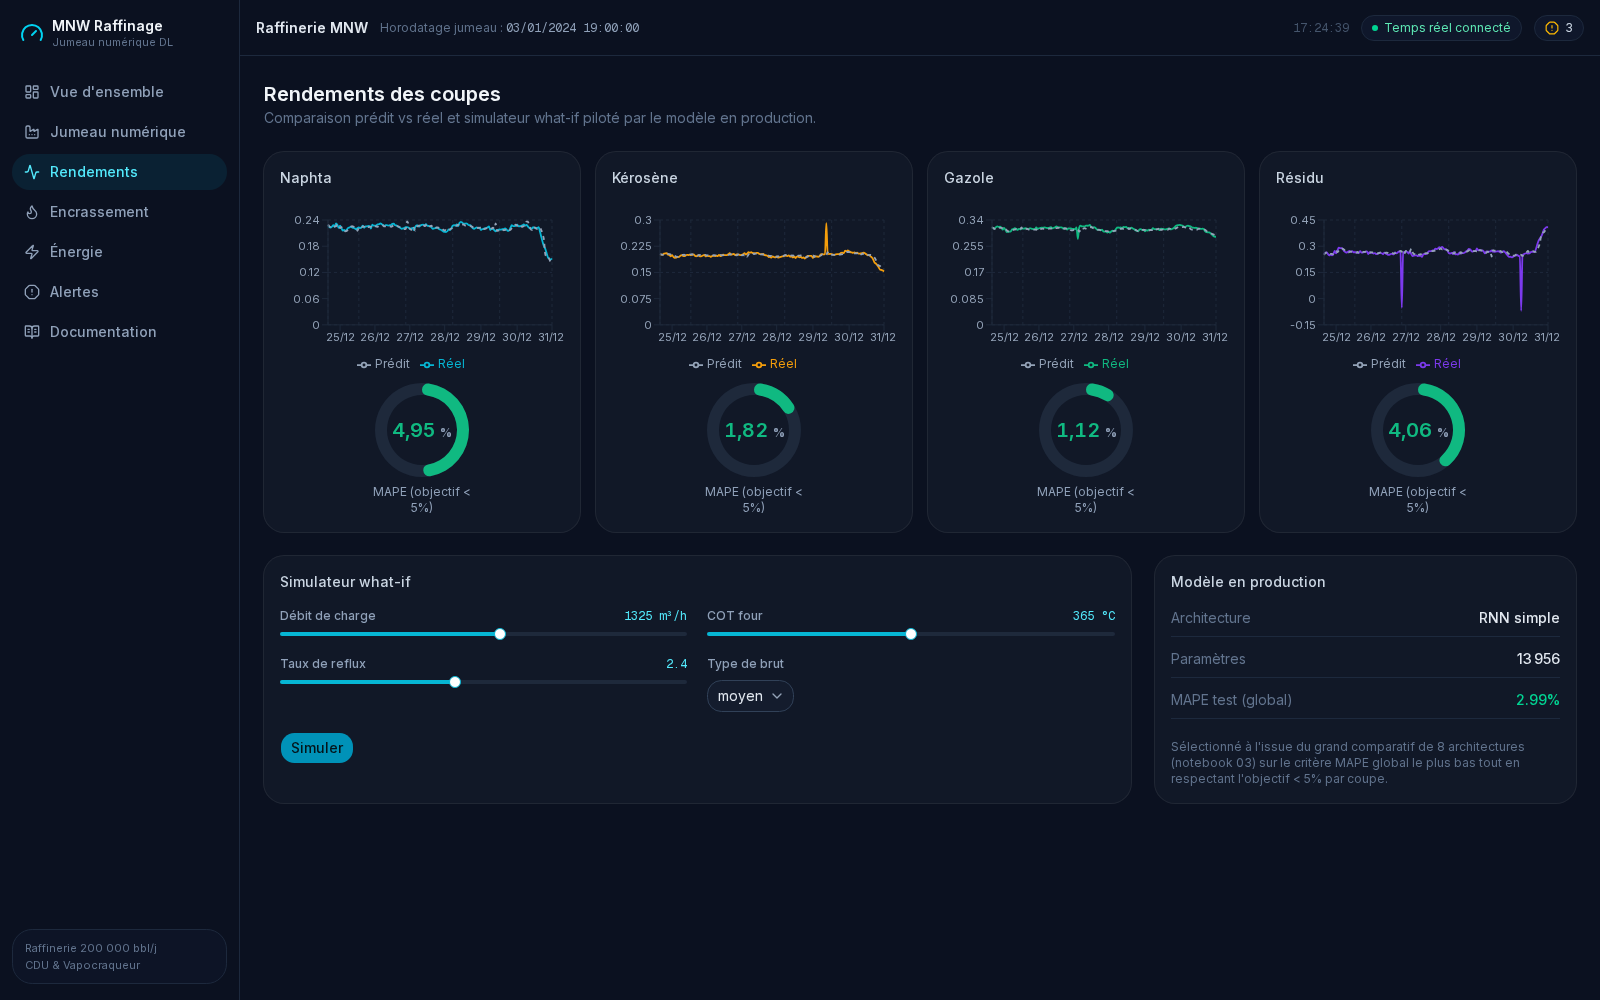
\includegraphics[width=0.85\textwidth]{dashboard_rendements.png}
\caption{Page rendements — prédit vs réel, simulateur what-if}
\end{figure}

\begin{figure}[h]
\centering
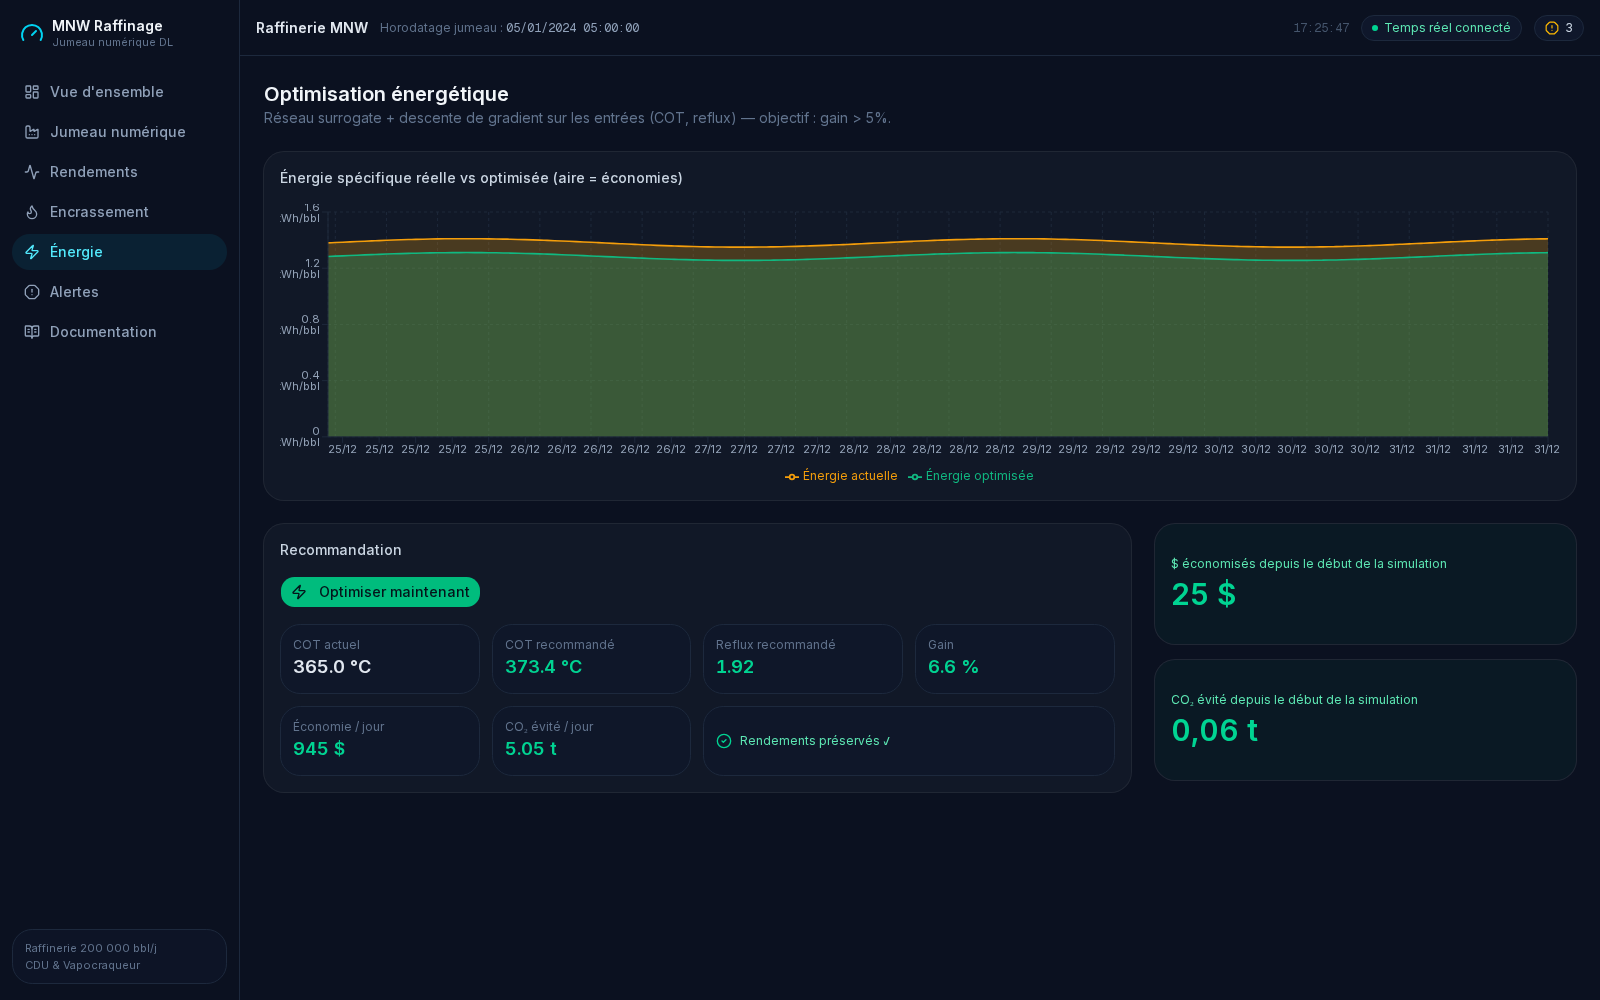
\includegraphics[width=0.85\textwidth]{dashboard_energie.png}
\caption{Page énergie — après optimisation à la demande}
\end{figure}

\section{Stack technique}

\begin{table}[h]
\centering
\begin{tabular}{p{2.5cm}p{4cm}p{7cm}}
\toprule
Composant & Technologie & Pourquoi \\
\midrule
Deep Learning & PyTorch, torchinfo, tqdm & Framework standard, flexible, CPU-friendly \\
Backend & FastAPI, Pydantic v2, uvicorn, WebSockets & Async natif, validation stricte, WebSocket intégré \\
Frontend & Next.js (App Router, TS) & Rendu hybride SSR/CSR, écosystème React mature \\
UI & Tailwind CSS, shadcn/ui & Composants accessibles, thème sombre rapide \\
Graphiques & Recharts & Déclaratif, natif React \\
Synoptique & @xyflow/react & Diagrammes de flux interactifs avec nœuds custom \\
État/Données & TanStack Query, zustand & Cache de requêtes + état global léger \\
Animations & framer-motion & Transitions déclaratives \\
Icônes & lucide-react & Icônes cohérentes, légères \\
Conteneurisation & Docker, docker-compose & Reproductibilité, isolation \\
Environnement Python & \texttt{uv} & Résolution rapide des dépendances \\
\bottomrule
\end{tabular}
\caption{Stack technique et justification}
\end{table}

\subsection*{Icônes à télécharger (facultatif)}

Le dashboard utilise \textbf{lucide-react} (icônes vectorielles intégrées, aucun téléchargement
nécessaire pour l'app). Pour illustrer ce rapport avec des logos de technologies (marques
déposées de leurs propriétaires respectifs) :
\begin{itemize}
  \item PyTorch : \url{https://pytorch.org/assets/images/pytorch-logo.png}
  \item FastAPI : \url{https://fastapi.tiangolo.com/img/logo-margin/logo-teal.png}
  \item Next.js : \url{https://nextjs.org/static/favicon/favicon-32x32.png}
  \item Docker : \url{https://www.docker.com/wp-content/uploads/2022/03/Moby-logo.png}
\end{itemize}

\section{Conclusion}

Les 5 objectifs métier sont atteints avec des réseaux de neurones uniquement, sur des données
100\% synthétiques mais physiquement cohérentes. Le meilleur modèle de rendements (RNN simple)
est volontairement le plus simple testé — illustration qu'une architecture plus complexe
n'est pas toujours nécessaire. Le pipeline complet tourne en quelques dizaines de millisecondes,
largement compatible avec un déploiement temps réel.

\end{document}
